\documentclass[answers, addpoints]{exam} % haal het `answers` weg voor een pdf met alleen de vragen.
\renewcommand{\solutiontitle}{\noindent\textbf{Solution}\par\noindent}
\pointpoints{point}{points}

\usepackage[english]{babel}
\usepackage{amsmath, amssymb, amsthm, enumitem}
\usepackage{mathtools, mathrsfs}
\usepackage{graphicx}
\usepackage{siunitx}
\usepackage{float}
\usepackage{hyperref}

\newcommand{\Bb}[1]{\mathbb{#1}}
\newcommand{\Bf}[1]{\mathbf{#1}}
\newcommand{\Cal}[1]{\mathcal{#1}}
\newcommand{\NN}{\mathbb{N}} % â„•
\newcommand{\ZZ}{\mathbb{Z}} % ℤ
\newcommand{\QQ}{\mathbb{Q}} % â„š
\newcommand{\RR}{\mathbb{R}} % ℝ
\newcommand{\CC}{\mathbb{C}} % â„‚
\newcommand{\PP}{\mathbb{P}} % â„™
\newcommand{\EE}{\mathbb{E}} % 𝔼
\DeclareMathOperator{\var}{Var} % Variantie
\DeclareMathOperator{\cov}{cov} % Covariantie
\newcommand*\diff{\mathop{}\!\mathrm{d}} %Gebruik als \int f(x) \diff x

% Kwestie van smaak:
\renewcommand{\epsilon}{\varepsilon}
\renewcommand{\phi}{\varphi}

% Gegevens
\title{Final exam Fundamentals of Photonics 2019/2020\\
      \large 25 maart 2020\footnote{This exam was probably meant as 2019's resit, which wasn't held.
It was used as 2020's final exam.}} % Datum van tentamen

\author{Siem de Jong\footnote{Altough these solution were written with care, I could've made mistakes. If you find one, please let me know.} \\ \href{mailto:siem.dejong@student.uva.nl}{siem.dejong@student.uva.nl}}
\date{\today} % Datum van uitwerken

\begin{document}

\maketitle

\part{Closed book questions}

\begin{questions}

  \question[5] For the first three questions select the correct answer from multiple choices and for the last two questions fill the correct answer in the blank area.
  
  \begin{parts}

    \part[1] The phase difference ($\phi$) and path difference ($\Delta L$) are related by $\phi = $  
    \begin{enumerate}
    \item[a] $\frac{2\pi}{\lambda}\Delta L$
    \item[b] $\frac{2\lambda}{\pi}\Delta L$
    \item[c] $\frac{\pi}{2\lambda}\Delta L$
    \item[c] $\frac{\lambda}{2\pi}\Delta L$
	\end{enumerate}    
    \begin{solution}
    	$\frac{2\pi}{\lambda} \Delta L.$
      Phase difference is a quantity with degrees or radians as units, so we can drop option b and d.
      Since a full wavelength is $2\pi$, we need answer a.
    \end{solution}

    \part[1] A phase difference $\pi$ between two interfering beams is equivalent to a path difference
	\begin{enumerate}
		\item[a] $\lambda$,
		\item[b] $\lambda/2$,
		\item[c] $\lambda/4$,
		\item[d] $\lambda/8$.
	\end{enumerate}	    
    \begin{solution}
      $\lambda/2$.
      Plug $\pi$ in the equation of the previous question and solve for the path difference.
    \end{solution}
    
    \part[1] When a light wave incident perpendicular to a surface is reflected at the surface of an optically denser medium, then the change in the phase difference is
    \begin{enumerate}
    \item[a] $\pi/2$,
    \item[b] $\pi/4$,
    \item[c] $\pi$,
    \item[d] $2\pi$.
    \end{enumerate}
    \begin{solution}
      ``The component of the electric field normal to the plane-of-incidence undergoes a phase shift of $\pi$ radians upon reflection when the incident medium has a lower index than the transmitting mdeium." If you'd like to get a mathematical explanation (using a Fresnel Equation), I suggest you read E. Hecht, \emph{Optics} (Harlow: Pearson Education Limited, 2017), 228.
    \end{solution}
    
    \part[1] If $D$ is the distance to the screen in Young's double slit experiment, then fringe width $\beta$ decreases with \underline{\hspace{3cm}} in $D$.
    \begin{solution}
      We have the relation
      \begin{displaymath}
      	\beta \approx \frac{m\lambda D}{d},
      \end{displaymath}
      where $m \in \mathbb{Z}$ and $d$ the distance between the slits.
      From this, we can state that $\beta$ decreases with \emph{decrease} in $D$.
    \end{solution}

	\part[1] If two waves maintain constant phase difference or equal phase at any two points on a wavefront is known as \underline{\hspace{3cm}}.
    \begin{solution}
      spatial coherence.
      Don't confuse spatial coherence with temporal coherence.
      Temporal coherence is a quantity which tells you how monochromatic a source is.
    \end{solution}

  \end{parts}

	\question[5] What is an optical mode in a waveguide/fiber? Sketch $m=0$, $m=1$, and $m=2$ modes in a symmetric slab waveguide.
	\begin{solution}
		An optical mode in a waveguide is the field pattern of propagating waves.
		In the next picture, the first three modes are illustrated.
		\begin{figure}[H]
			\centering
			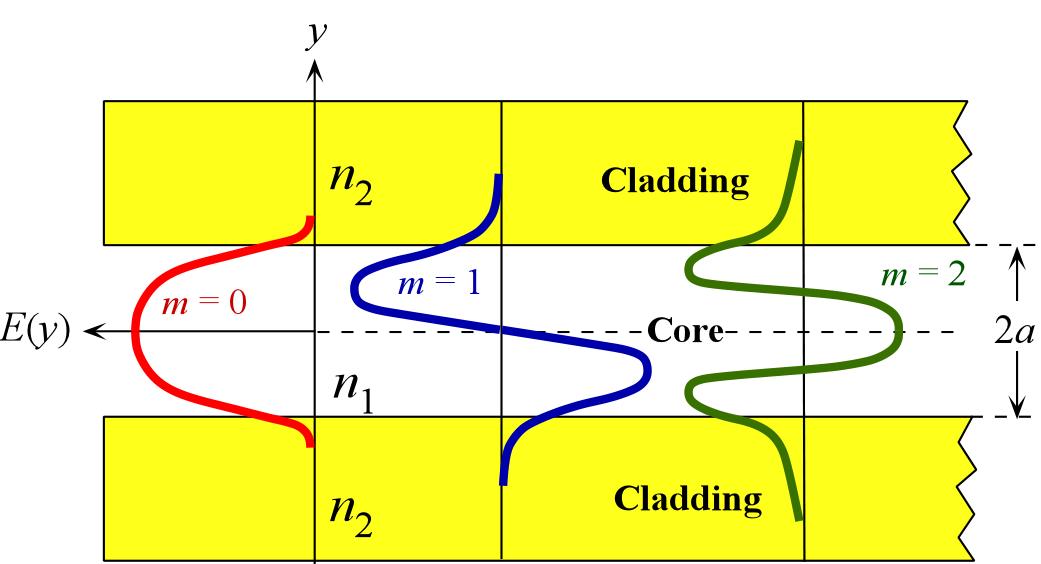
\includegraphics[scale=.5]{figures/wgmodes}
		\end{figure}
		Optical modes can have it's electric field or magnetic field entirely transverse.
		These modes are then called TE or TM modes respectively.
	\end{solution}

	\question[5] One of the methods to couple input light into an optical waveguide is prism coupling where you place a glass prism on top of the optical waveguide. Explain why a prism is needed in this configuration?
	\begin{figure}[H]
		\centering
		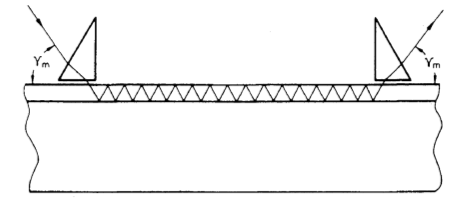
\includegraphics[scale=1]{figures/prismcoupling}
	\end{figure}
	\begin{solution}
		In an optical waveguide, we need light to undergo total internal reflection to make it propagate to the other side of the guide.
		If the light comes in at $\gamma_m$ (fixed) and has to go out at $\gamma_m$, then we need the prisms to assure the light is coming in the waveguide at such an angle that the internal reflections occur at the critical angle to prevent loss of the light.
		At the end, a prism is needed to get the light out of the waveguide and turn the evanescent wave of the total internal reflection into a propagating wave at angle $\gamma_m$.
		
		A prism also makes alignment of the beam and film easier without having to deal with very small precision.
		With a prism, the numerical aperture also doesn't have to match between the beam and the film.
		Using a prism coupler, the coupled beam can be much wider than the thickness of the waveguide.
	\end{solution}

	\question[5] What is index of refraction? How does it change with the wavelength of light? Assume normal dispersion regime.
	\begin{solution}
		Refractive index $n$ describes how fast light travels through a medium as it's relation is $n = \frac{c}{v}$, where $v$ is the measured speed.
		It effectively changes when the wavelength changes:
		\begin{displaymath}
		n_{\mathrm{effective}} = \frac{2\pi}{\lambda} n.
		\end{displaymath}
		If $\lambda$ gets bigger, the effective refractive index gets smaller.
	\end{solution}
	
	\question[5] In an optical microscope, if we change the objective lens to an objective lens with a higher numerical aperture, how does the beam waist and depth of focus change?
	\begin{solution}
		An optical microscope makes use of guassian beam.
		Here's an illustration of such a beam.
		\begin{figure}[H]
			\centering
			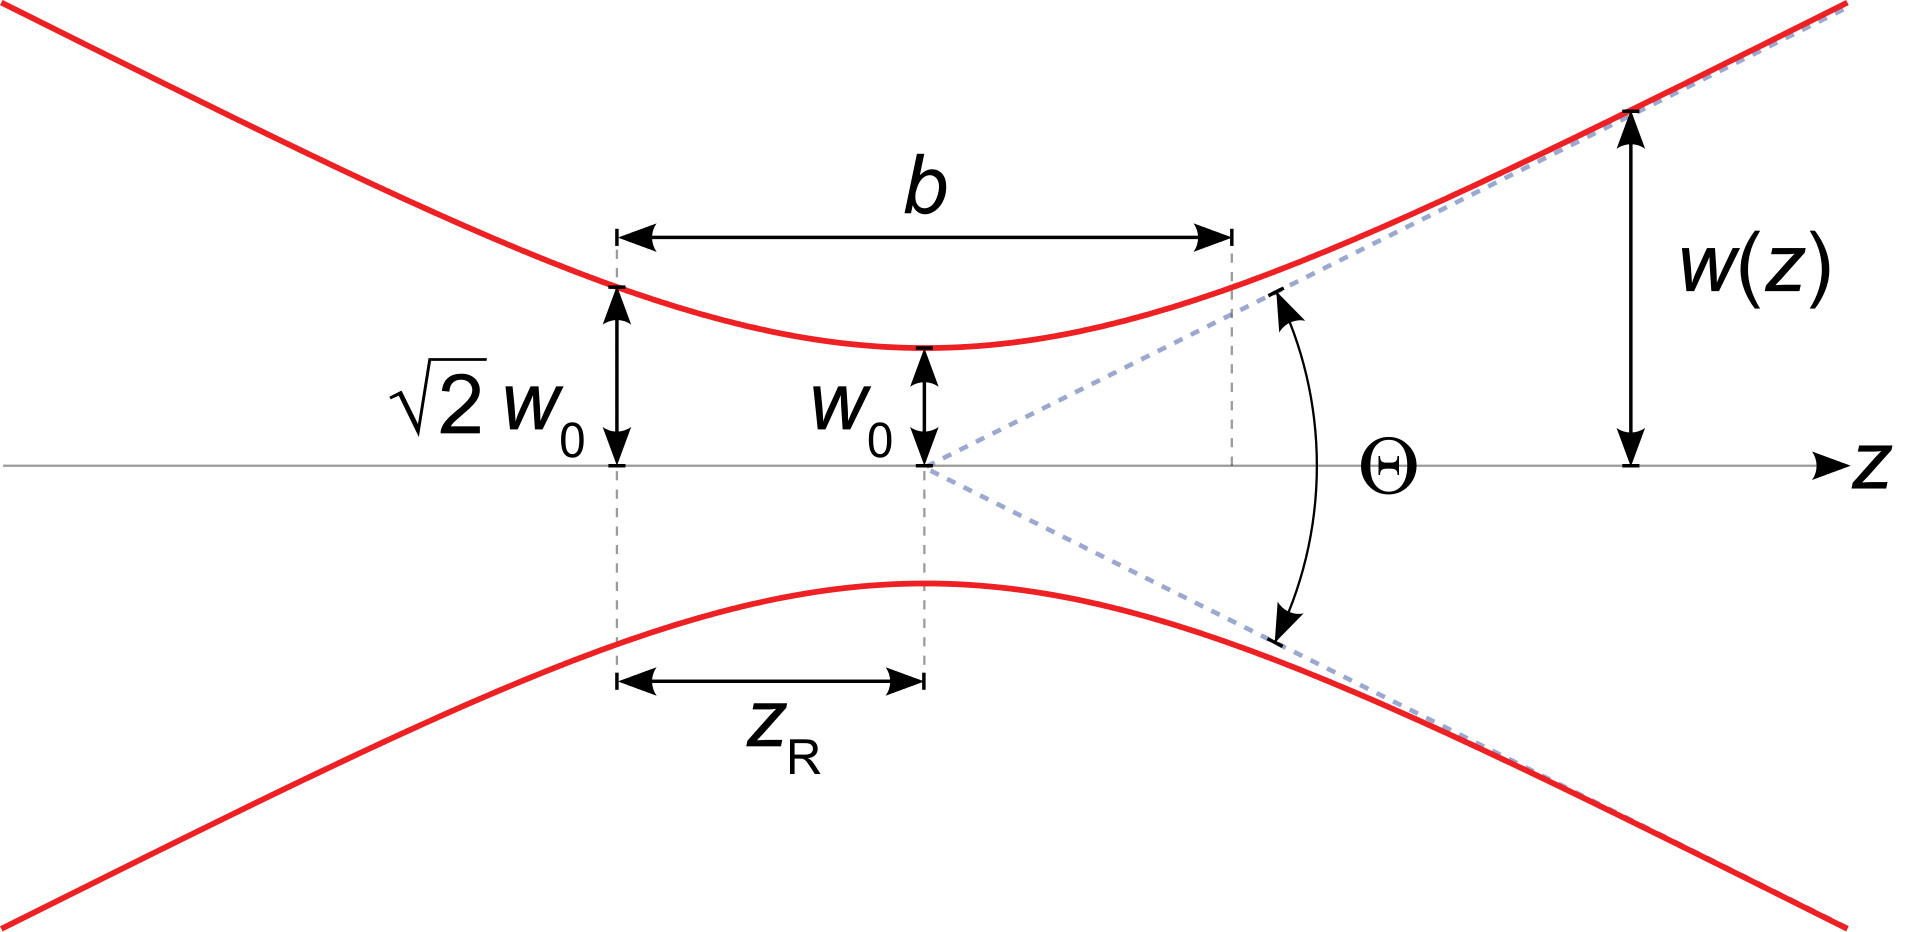
\includegraphics[scale=.1]{figures/gaussian}
		\end{figure}
		$b$ is the depth of focus and is related to the numerical aperture $\mathrm{NA}$ by $b=2 n w_0 / \mathrm{NA} = 2 Z_R$.
		So with a higher $\mathrm{NA}$, the depth of focus gets smaller.
		Also, $w_0$ is considered the beam waist and is roughly related to $\mathrm{NA}$ by $w_0 \propto \frac{1}{\mathrm{NA}}$, which results in a smaller beam waist if the numerical aperature gets higher.
	\end{solution}
		
	\question[5] A beam of light with intensity $I_0$ passes through two linear polarizers as shown above. The intensity of the final beam is $1/8 I_0$.
	Write down one possible polarization state of the input light that can result in this power output.
	\begin{figure}[H]
		\centering
		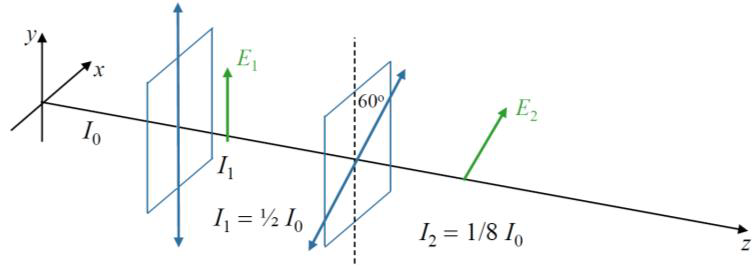
\includegraphics[scale=1]{figures/polarizers}
	\end{figure}		
	\begin{solution}
		For this questoin we need Malus' law:
		\begin{displaymath}
			I_1 = I_0 \cos^2\theta_i.
		\end{displaymath}
		Solve for $\theta$:
		\begin{align*}
			\frac{1}{2}I_0 &= I_0 \cos^2\theta \\
			\theta &= \arccos\frac{1}{\sqrt{2}} \\
			&= \SI{45}{\degree}.
		\end{align*}	
		So we need linearly polarized light at angle \SI{45}{\degree}.
	\end{solution}

\newpage
\part{Open book questions}
\setcounter{question}{0}

\begin{figure}[H]
	\centering
	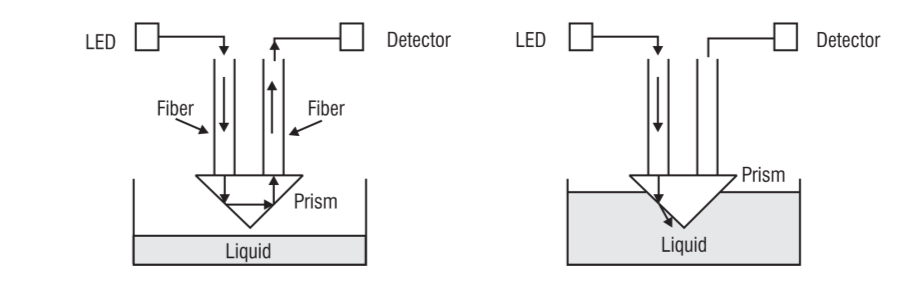
\includegraphics[scale=1]{figures/liquidsensor}
\end{figure}
\question[10] Above you see a liquid level sensor, which is comprised of two fibers and a prism.
Explain the working principle of this system.
\begin{solution}
	In the left picture, we see that the light reflects and transmits at a glass-air interface, for example.
	Some of the light reflects to the right and then up and some of the light transmits into the air.
	The detector measures the intensity.
	
	Now, in the right image, the prism is submerged in the liquid, meaning other portions of the light will reflect and transmit according to the Fresnel equations.
	The detector will measure a lower intensity as the light will leak out more at the prism interfaces when put in liquid than in air.
	If the difference is significant, the user will be notified.
	To see this sensor in action, take a look at this video: \url{https://youtu.be/ZByijUX_TDY}.
\end{solution}

\question[15] An unpolarized light with an intensity of $I_0$ is incident on two linear polarizers (\SI{45}{\degree} and \SI{60}{\degree}) and a quarter-wave plate (QWP).
\begin{figure}[H]
	\centering
	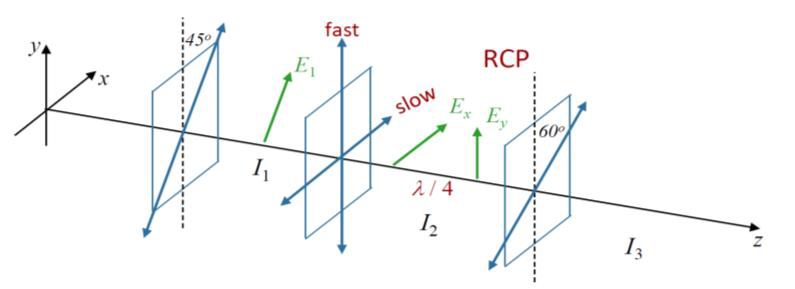
\includegraphics[scale=1]{figures/polarizers2}
\end{figure}
\begin{parts}
	\part What is $I_1$ in terms of $I_0$?
	Explain your answer.
	\begin{solution}
		Unpolarized light contains polarized light in all possible directions.
		When using Malus'law to calculate $I_1 = I_0\cos^2\theta$, we need to know the average of $\cos^2\theta$, because we want to know what happens to `each polarized part in the unpolarized light'.
		To calculate the average of $\cos^2\theta$ we have
		\begin{align*}
			\sin^2\theta + \cos^2\theta = 1.
		\end{align*}
		If we take the average of this equation, we get
		\begin{align*}
			\langle\sin^2\theta\rangle + \langle\cos^2\theta\rangle = \langle 1\rangle = 1.
		\end{align*}
		Because  $\langle\sin^2\theta\rangle = \langle\cos^2\theta\rangle$, we can state that $\langle\cos^2\theta\rangle = \frac{1}{2}$. So $I_1 = \frac{1}{2}I_0$.
	\end{solution}
	\part What is the polarization state of the light after the QWP?
	\begin{solution}
		Quarter wave plates make circular polarized light of polarized light.
		So circularly polarized.
	\end{solution}
	\part What is the intensity of light $I_2$ after the QWP?
	\begin{solution}
		Waveplates don't alter the intensity of incoming light.
		So $I_2 = I_1 = \frac{1}{2}I_0$
	\end{solution}
	\part Assume that $E_0 = E_0\sin(kz-\omega t)$
	Write down $E_x$ and $E_y$ in terms of $E_1$ after the QWP.
	\begin{solution}
		The $x$ part of the wave gets retarded and thus a little extra phase of \SI{90}{\degree}.
		We then have
		\begin{align*}
			E_y &= E_0 \cos\left(k z - \omega t\right) \\
			E_x &= E_0 \cos\left(k z - \omega t + \frac{\pi}{2}\right),
		\end{align*}
		assuming we need to write $E$ in terms of $E_0$ instead of $E_1$.
		If not, then
		\begin{align*}
			E_y &= E_1 \\
			E_x &= E_1 \frac{\sin\left(k z-\omega t + \frac{\pi}{2}\right)}{\sin\left(k z -\omega t\right)} \\
			&= E_1 \cot\left(k z - \omega t\right).
		\end{align*}		
	\end{solution}
	\part What is the polarization state of the light after the \SI{60}{\degree} polarizer?
	\begin{solution}
		All the light other than at \SI{60}{\degree} will be blocked, resulting in linearly polarized light at \SI{60}{\degree}.
	\end{solution}
	\part If we replace the \SI{60}{\degree} polarizer with another QWP with the fast axis oriented along the $x$ direction and the slow axis along the $y$ direction, what will be the polarization of the light after the second QWP?
	\begin{solution}
		The $E_y$ part will be retarded by $+\frac{\pi}{2}$ phase making the phase difference between the $y$ and $x$ part zero, polarizing it again to \SI{45}{\degree}.
		The circular polarization gets undone.
	\end{solution}
	\part What will be the intensity of the light after the second QWP in terms of $I_1$?
	\begin{solution}
		QWPs don't alter the intensity, thus the intensity will be $I_3 = I_2 = I_1 = \frac{1}{2}I_0$.
	\end{solution}
\end{parts}

\question[10] Below two electromagnetic waves with same frequency and different field amplitudes are given.
\begin{align*}
	E_1 &= E_{10}\sin(\omega t) \\
	E_2 &= E_{20}\sin(\omega t + \phi)
\end{align*}
If these two waves superimpose ate a point $P$, show that the intensity at $P$ is $I = I_1 + I_2 + 2\sqrt{I_1I_2}\cos(\phi)$.
\begin{solution}
	First, we change the notation to it's complex form.
	\begin{align*}
		E_1 &= E_{10}\sin(\omega t)= E_{10}\cdot\Im{\left(e^{i\omega t}\right)} \\
		E_2 &= E_{20}\sin(\omega t + \phi) =E_{20}\cdot\Im{\left(e^{i\omega t + \phi}\right)}
	\end{align*}
	When we calculate the intensity, we need to add the fields up before squaring.
	\begin{align*}
		I &= (E_1+E_2)^2 \\
		&= \left[E_{10}e^{i\omega t} + E_{20}e^{(\omega t +\phi)}\right]^2 \\
		&= \left[e^{i\omega t}\right]^2 \left[E_{10}+E_{20}e^{i\phi}\right]^2 \\
		&= E_{10}^2+E_{20}^2+2E_{10}E_{20}e^{i\phi} \\
		&= I_1+I_2+2\sqrt{I_1I_2}\cos\phi
	\end{align*}
	We take the real part of the complex term in the last step and take $I_{i} = E_{i0}^2$.
	Note that squaring a complex number means multiplying by it's complex conjugate, e.g. $\left|e^{i\phi}\right|^2 = e^{i\phi}e^{-i\phi} = 1$.
\end{solution}

\question[10] Waveguide coupler
\begin{figure}[H]
	\centering
	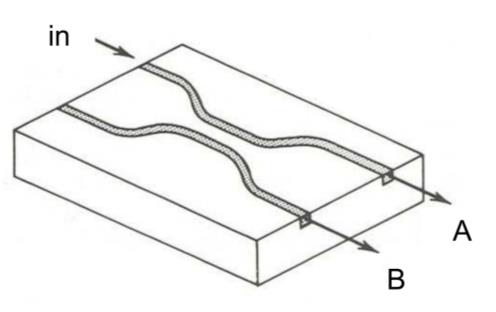
\includegraphics[scale=1]{figures/coupler}
\end{figure}
\begin{parts}
	\part[3] Explain the general operating principle of the waveguide coupler shown above.
	\begin{solution}
		A waveguide coupler brings two waveguides close to eachother.
		Because of this, the evanescent field from one light out of the other waveguide gets into the other waveguide and can propagate further until it hops to the other waveguide again.
		This hopping of the light occurs until the end of the coupler.
		Because the two waveguides are close to each other, we say they are coupled.
		If the two waveguides were single mode, then the collection is a two-mode structure and there's an antisymmetric and symmetric mode.
		\begin{figure}[H]
			\centering
			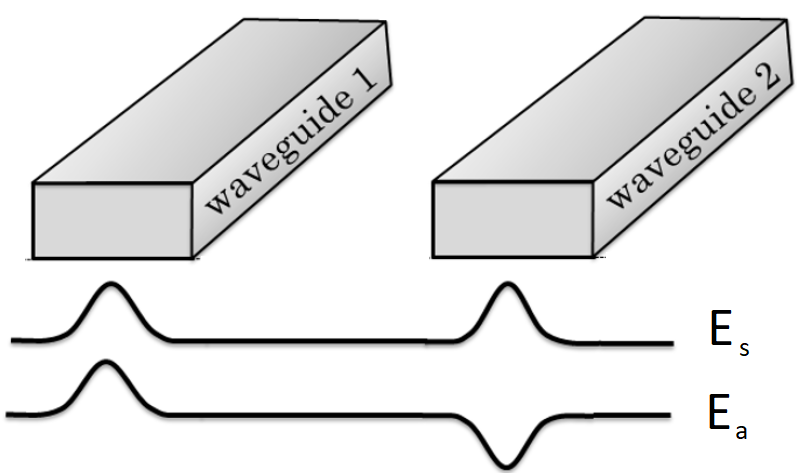
\includegraphics[scale=.5]{figures/modesincoupler}
		\end{figure}
	\end{solution}
	\part[2] Explain how the waveguide coupler can be used to split the incoming signal in two equal output signals A and B.
	\begin{solution}
		Because of the hopping nature of the structure, the light can be partly in one of the waveguides.
		If this part of the light is equal to the other part in the other waveguide, then we can stop the coupling there and the output signals at A and B are equal.
		\begin{figure}[H]
			\centering
			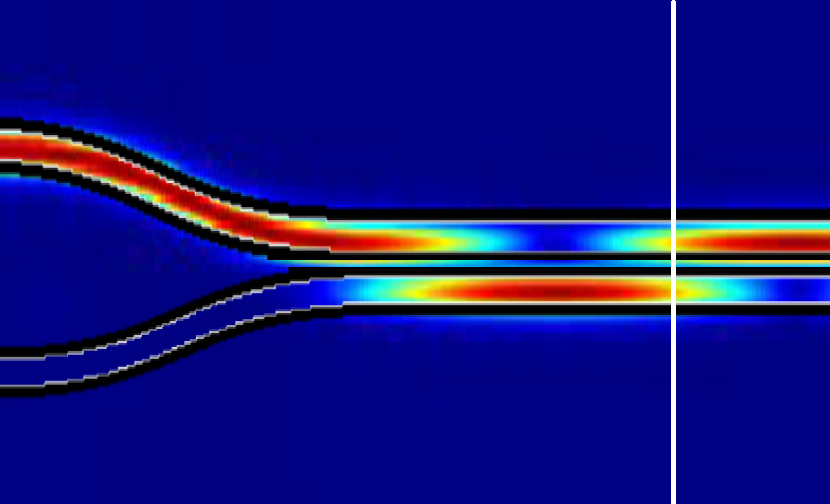
\includegraphics[scale=.5]{figures/hopping}
		\end{figure}
	\end{solution}
	\part[2] In order to make the coupling ratio variable, what kind of a mechanism can be used?
	\begin{solution}
		It is possible to make the coupling ration variable if we make use of electro-optic material in the place of the coupler.
		When an electric field is applied to this material, the optical path changes, which results in a different distribution of light at the output.
	\end{solution}
	\part[3] If we increase the width of waveguide B, how would this change the device performance?
	\begin{solution}
		This makes the waveguide asymmetric.
		The light will never fully escape waveguide B and if the increase in width of B is big enough, the power in A will never be higher than B.
		In that case, it's also not possible to have the two outputs be exactly the same.
		\begin{figure}[H]
			\centering
			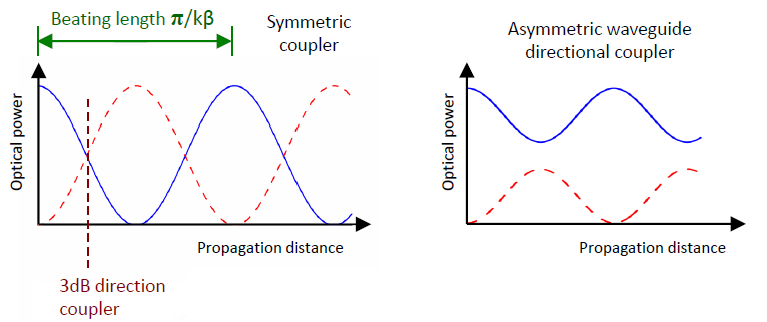
\includegraphics[scale=.8]{figures/symmetriccoupler}
		\end{figure}
		Also, if B is wide enough, then it won't be single mode, so there will be more scattering in the core which is not desirable.
	\end{solution}
\end{parts}

\question[10] White light in air shines on an oil film that floats on water with an incident angle of \SI{90}{\degree} as shown below.
When looking straight down at the film, the reflected light is red, with a wavelength of \SI{636}{\nano\meter}.
What is the minimum possible thickness of the film?
\begin{figure}[H]
	\centering
	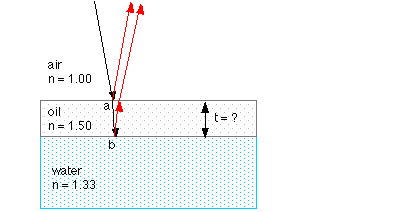
\includegraphics[scale=1]{figures/oilfilm}
\end{figure}
\begin{solution}
	White light contains a continious spectrum of wavelengths, but if we only want to have constructive interference after reflection, we have to meet the constructive interference condition for $\lambda=\SI{636}{\nano\meter}$.
	The air and the water both have lower refractive indices than oil, so at the first reflection there will be a $\pi$ phase shift.
	At the second there won't be one.
	%TODO SKETCH REFLECTIONS
	We got
	\begin{align*}
		2 n_{\mathrm{oil}} t_m &= \left(m+\frac{1}{2}\right)\lambda \\
		t_m &= \frac{1}{2n_{\mathrm{oil}}}\left(m+\frac{1}{2}\right)\lambda.
	\end{align*}
	The minimum possible thickness is then
	\begin{align*}
		t_0 &= \frac{1}{2}\frac{1}{2}\frac{636}{1.5}\si{\nano\meter} \\
		&= \SI{106}{\nano\meter}.
	\end{align*}
\end{solution}

\question[15] Sketch a time-domain optical coherence tomography (OCT) system based on the next interferometers.
On your schematic write down each components' name explicitly and mention their function.
\begin{parts}
	\part Mach Zehnder interferometer (MZI)
	\begin{solution}
		\begin{figure}[H]
			\centering
			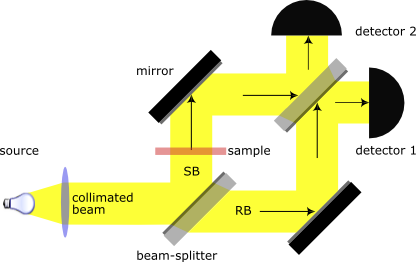
\includegraphics[scale=.5]{figures/mzinterferometer}
		\end{figure}
		If there's no sample then the two beams will constructively interfere at detector 1 and destructively interfere at detector 2.
		If we put a sample inside the left beam, this sample beam will be slightly phaseshifted and thus there will be different interference patterns at the detector.
		From this, it's possible to deduce the phase shift caused by the sample.
	\end{solution}
	\part Michelson interferometer (MI)
	\begin{solution}
		\begin{figure}[H]
			\centering
			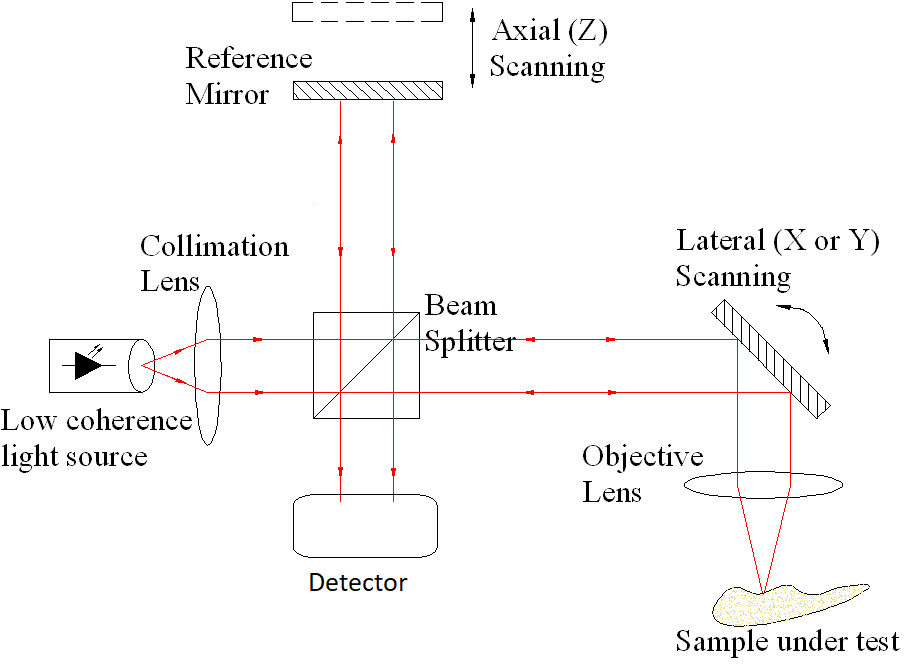
\includegraphics[scale=.5]{figures/minterferometer}
		\end{figure}
		Here we have a low coherent light source going through a collimating lens so we can bounce the light useful off mirrors.
		The beam gets split to the sample and a reference arm.
		The beam to the reference arm can be rotated so different points of the sample get imaged.
		The reference mirror will move to see how the interference at the detector is changed.
	\end{solution}
	\part What is the advantage of using an MZI compared to MI? Indicate the additional components that are needed to configure an MZI based OCT.
	\begin{solution}
		In the MZI each path is only taken once, which doesnt allow particles going in opposite directions interact strangely with each other as in the MI.
		For MZI we need one detector more and one more beam splitter.
		When using the MI, part of the light goes back to the light source which can't be used.
	\end{solution}
	\part If one needs to build an ultra-high resolution OCT system (axial resolution $\sim$ \SI{1}{\micro\meter}), what kind of a light source will be needed? What is the biggest challenge of an ultra-high OCT system?
	\begin{solution}
		The axial resolution is
		\begin{align*}
			l_\mathrm{c} \approx 0.44 \frac{\lambda_0^2}{\Delta \lambda},
		\end{align*}
		so the higher the bandwidth, the shorter the coherence length resulting in a higher resolution.
		Maximizing this bandwidth is the biggest challenge nex to lowering $\lambda_0^2$ as much as possible.
		When $\lambda_0$ gets very small, very much energy is required.
	\end{solution}
\end{parts}
\end{questions}

\end{document}
